
%!TEX TS-program = xelatex
%!TEX encoding = UTF-8 Unicode

\documentclass[12pt]{article}
\usepackage{geometry}                % See geometry.pdf to learn the layout options. There are lots.
\geometry{letterpaper}                   % ... or a4paper or a5paper or ... 
\usepackage{amsmath}
\usepackage{graphicx}
\usepackage{amssymb}
\usepackage{framed}
\usepackage{listings}
\lstset{language=Octave,
  basicstyle=\footnotesize,
  tabsize=3,
  language=python,
  breaklines=true,
  mathescape=true,
  commentstyle=\color{blue},
  morecomment=[l]{\#}}
\usepackage{fontspec,xltxtra,xunicode}
\defaultfontfeatures{Mapping=tex-text}
\setromanfont[Mapping=tex-text]{Hoefler Text}
\setsansfont[Scale=MatchLowercase,Mapping=tex-text]{Gill Sans}
\setmonofont[Scale=MatchLowercase]{Andale Mono}

\author{Elliott Hauser}
\title{Comp 555 Problem Set 4}
\begin{document}
\maketitle
\section*{Question 1}
\subsection*{a}  While both Hash-table and Suffix trees would correctly solve this problem, they may be preferred over one another depending on the circumstances.  Suffix trees have a run time of $O(m)$, making them preferable \textit{ceteris paribus}.  But there is computational and engineering overhead to generate the suffix tree. Hash tables are implemented natively in many programming languages (such as Python's \lstinline{dict} structure), making them easier to implement in some situations.

That said, for our purposes computational and engineering overhead are negligible when compared to runtime savings, especially given that $n$ is likely to be very long.  So, the suffix tree structure is most appropriate for our purposes here.

\subsection*{b} Assuming the suffix table for $m$ is already constructed as a graph, an algorithm to find the number of occurrences of $m$ in $n$ is given in Figure~\ref{suffsearch}
\begin{figure}[ht]
\begin{framed}
\begin{lstlisting}

Preprocess $n$ into suffix tree $s_n$ in $O(n)$.

SuffixSearch($m$, $s_n$)
position = 0
for edge in childEdge($s_n$) == $m$[position:len(edge_label)]
	if descendent vertex has child edge == $m$[position +1:len(child_edge_label)]
		SuffixSearch($m$[position+1:len($m$)], descendants(edge)
	else
		matches = count(descendants(edge))
		return matches

\end{lstlisting}
\end{framed}
\caption{An algorithm to find a string $m$ in a longer string $n$.}
\label{suffsearch}
\end{figure}

\subsection*{c}  The time complexity is $O(m)$.
\clearpage
\section*{Question 2}
A hash table scheme for providing the student id, given a score $x$, is to sort student IDs into a Hash table based on some feature of the scores themselves.  For this problem, we've been told that the scores can range from -10 to 20 and that the hash table should have at most 5 rows.  There are many solutions to this, but an optimal solution would divide both possible and actual values as evenly as possible amongst the 5 rows to reduce collisions.  The best solution I've found is to separate scores based on the sum of their digits.  Table~\ref{hashintro} illustrates where each possible score would be stored.  This scheme achieves the goal of equally distributing possible values of scores across the rows.  In addition, as shown below in b, the actual values of scores are distributed evenly, $+/- 1$ score.  Within rows, values should be ordered by ascending score.-

\begin{table}[h]
\centering
\begin{tabular}{c|l}
Digit sums & Corresponding scores\\\hline
$1, 2$ & $-2,-1,1,2,10,11$\\
$3,4$ & $-4,-3,3,4,12,13$\\
$5,6$ & $-6,-5,5,6,14,15$\\
$7,8$ & $-8,-7,7,8,16,17$\\
$9,10,0$ & $-9,0,9,10,18,19$\\
\end{tabular}
\caption{A hash table scheme for storing student IDs and scores based on the sum of the digits of the score.  Each row has six possible scores.}
\label{hashintro}
\end{table}


\subsection*{a} The hash function in Figure~\ref{digithash} shows a hash function to construct and populate the table described in Table~\ref{hashintro}.
\begin{figure}
\begin{framed}
\begin{lstlisting}[language=python, mathescape=true]

MakeTable()
# Makes a blank table
hash_table = 2 columns x 5 rows

# Add digit counts
for row, count in hash_table, range(1,9,2)
	row[0] $\gets$ [count, count+1]

# Add zero
hash_table[5][0] $\gets$ 0

DigitHash(score)
# Adds the digits of a score
for digit in score
	sum += abs(digit)	
return sum

AddStudent(student,x)
# Adds student and score to table in correct spot
sum = DigitHash(x)

for row in hash_table where row[0] == sum
	# if there's already a student with that score, add this student
	if row[1][0] == sum
		row[1] $\gets$ student
	# otherwise, make a new entry with score and student.
	else
		add \{sum, student\} to row[1]

\end{lstlisting}
\end{framed}
\caption{A digit sum hash function.}
\label{digithash}
\end{figure}

\subsection*{b} 
The actual hash table for this question is shown in Table~\ref{hashintro}.  As noted above, the scheme achieves a relatively even distribution of scores, minimizing collisions.  Even though Row 2 has three students in it, and Row 1 only has one, there is no way to reduce collisions further in a hash table this small.
\begin{table}[h]
\centering
\begin{tabular}{c|l}
Digit sums & Corresponding scores\\\hline
$1, 2$ & \{-1,A4\}\\
$3,4$ & \{4,A1,A2\},\{12,A8\}\\
$5,6$ & \{14,A5\},\{15,AA\}\\
$7,8$ & \{7,A9\},\{17,A7\}\\
9,10,0 & \{9,A3\},\{19,A6\}\\
\end{tabular}
\caption{The actual hash table for Question 2.}
\label{hashintro}
\end{table}


\subsection*{c} The script in Figure~\ref{script} would return the two students with a score of four. 
\begin{figure*}[h]
\centering
\begin{framed}
\begin{lstlisting}
index = DigitHash(4)   			# =>  4

for row[0] in hash_table == index  	# =>  2nd row
	Find 4 in entry in row[1]		# =>  first item
	return entry[1::]				# =>  [A1, A2]
\end{lstlisting}
\end{framed}
\caption{Locating all students with score of 4 using my hash table.}
\label{script}
\end{figure*}

\clearpage
\section*{Question 3}  An algorithm to find all palindromes of length 2 or greater is in Figure~\ref{palindromes}.  This algorithm is $O(nm)$, where $n$ is the length of the string being searched and $m$ is the average length of palindromes found.

A more efficient method would be to simultaneously search two suffix trees, one of the string, and one of its reverse.  This method would involve seeking mirror image patterns in the trees and then searching for the total pattern.  A rough sketch of this approach is in Figure~\ref{suffindrome}.

\begin{figure}[h]
\centering
\begin{framed}
\begin{lstlisting}
PalindromeSearch(text)
"""Find & return all palindrome strings in a text"""

palindromes = [ ]

for n in len(text)
	if nth char in text equals (n+1)^{th} char
		palindromes $\gets$ PalindromeBuild(n, n+1, text)
	if nth char in text equals (n+2)^{th} char
		palindromes $\gets$ PalindromeBuild(n, n+2, text)

return palindromes


PalindromeBuild(start, stop, text)
"""Takes the start and stop positions of a palindrome in a text.  Extends palindrome found between start and stop, if possible, and returns longest palindrome found"""
if text[start-1] == text[stop+1]
	PalindromeBuild(start-1,stop-1)
else 
	return text[start:stop]
\end{lstlisting}
\end{framed}
\caption{An algorithm to find all palindromes in a text in O(n) on the length of the text.}
\label{palindromes}
\end{figure}

\begin{figure}[h]
\begin{framed}
\begin{lstlisting}
# Assume we have suffix trees of both the string and its inverse

suffix = suffix tree of string
prefix = suffix tree of reverse of string

depth = 1
candidates = [ ]
path = [ ]

SuffixSearch(suffix, prefix)
RecurTree(suffix, prefix, depth)
	(returns candidates)
	
For path in candidates
	thread path through suffix
		when thread breaks, return path_traveled.

def RecurTree(suffix, prefix, depth, path)
	For each node at depth in suffix
		follow path through prefix
		if prefix has a node at end of path equal to suffix node
			path $\gets$ node
			depth +1
			RecurTree(suffix, prefix, depth, path)
		candidates $\gets$ path
\end{lstlisting}
\end{framed}
\caption{A sketch of the suffix tree approach to finding palindromes in a string.}
\label{suffindrome}
\end{figure}


\clearpage
\section*{Question 4}
%Use Agglomerative Hierarchical Clustering
\subsection*{a} A distance matrix is given in Table~\ref{eudistance}
\begin{table}
\centering
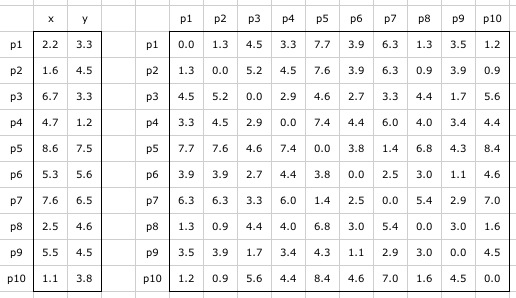
\includegraphics[width=4in]{eudistance.jpg}
\caption{A Euclidean distance matrix.}
\label{eudistance}
\end{table}

\subsection*{b \& c}
% need to fix hierarchical clustering

% Distance is maximal between pairs
\begin{figure}
\centering
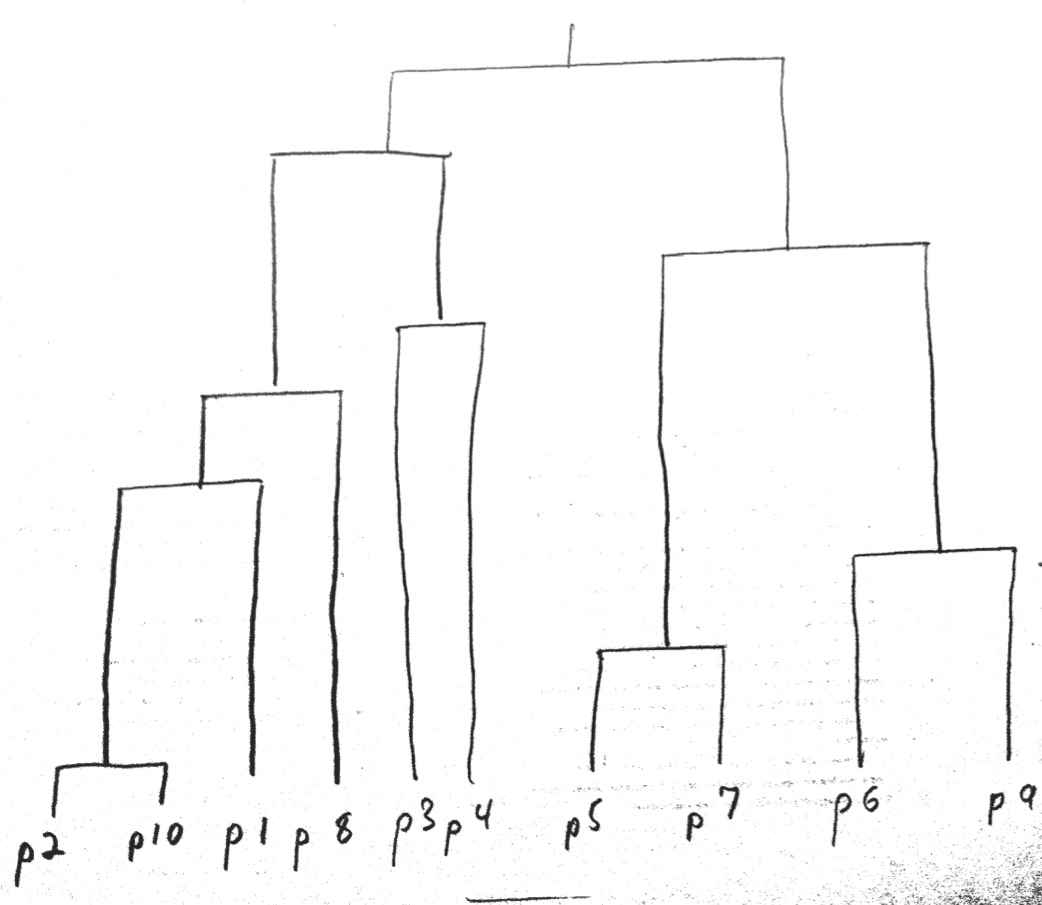
\includegraphics[width=2.25in]{maxtree.jpg}
\hspace{1cm}
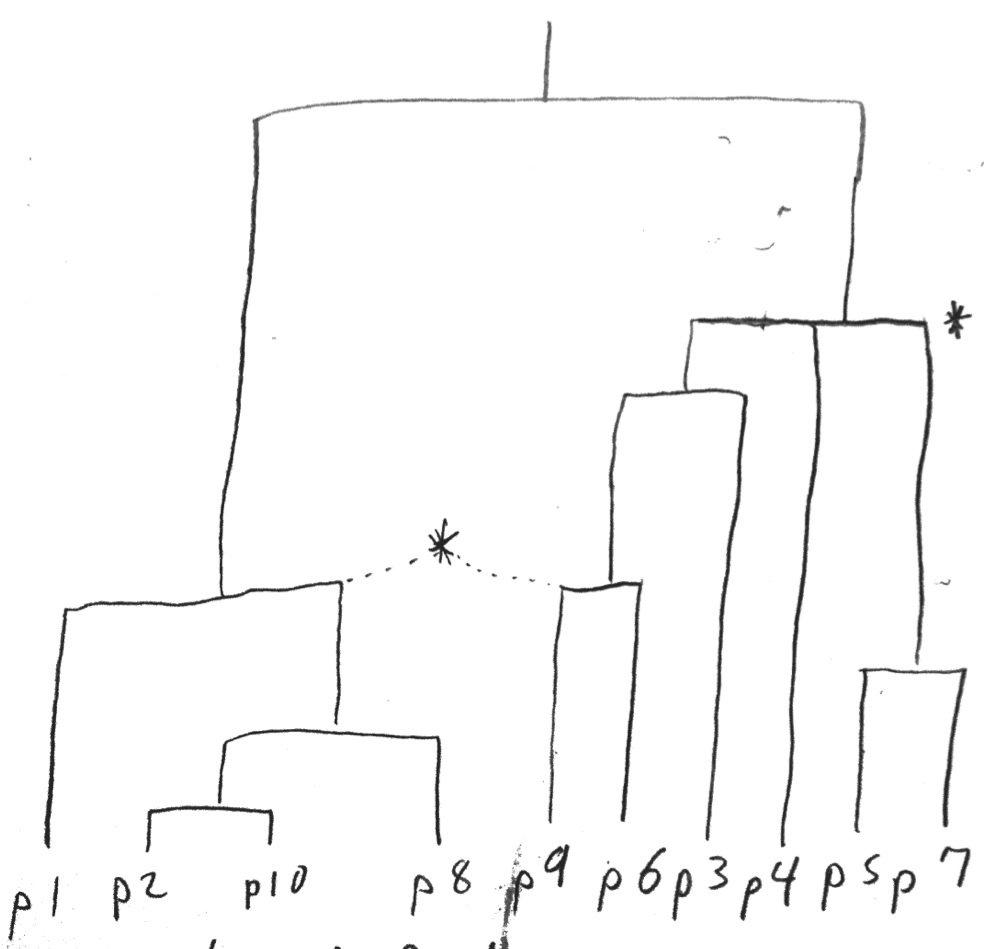
\includegraphics[width=2.25in]{mintree.jpg}
\caption{Maximum (right) and minimum (left) distance hierarchical agglomerative clusters.}
\label{trees}
\end{figure}
In constructing these trees, it seemed that the minimal distance pairs were much easier to construct from the distance matrix.  That said, the actual tree was less expressive.  As you can see at the points starred in Figure ~\ref{trees}, there were several 'collisions', where the minimum distances were identical for more than one pair of clusters.  This makes the tree less expressive than the maximum distance tree.  On the other hand, the greatest distance tree seemed to penalize much more for outliers.  It seems prudent to utilize centroids in many cases to mitigate these shortcomings.

\subsection*{d \& e}  Figure~\ref{kcharts} shows k-means clustering schemes for two different initial points.  As you can see, both sets of initial cluster representatives yield the same clustering once equilibrium is reached.  The k-means algorithm is robust to poor choices of cluster representatives, but picking sensible initial points could significantly reduce run times.

\begin{figure}[h]
\centering
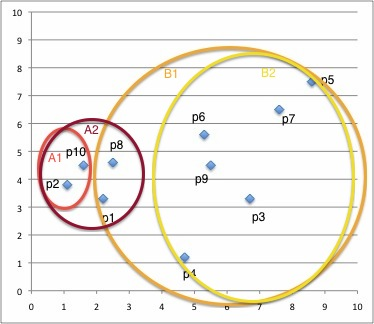
\includegraphics[width=2.25in]{chart12.jpg}
\hspace{1cm}
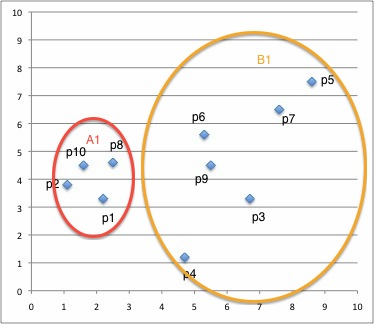
\includegraphics[width=2.25in]{chart910.jpg}
\caption{k-means clustering using p1 and p2 (left) and p9 and and p10 (right) as initial cluster representatives.  Both sets of parameters converge into identical clusters A and B.}
\label{kcharts}
\end{figure}
% could use more attention
\clearpage
\section*{Question 5}
\subsection*{1} The substrings were taken from \lstinline{crYsubset.fa}.  I generated random 'slices' of this text of length 100 characters 500 times to generate the data below.


\subsection*{2}
\begin{figure}[h]
\centering 
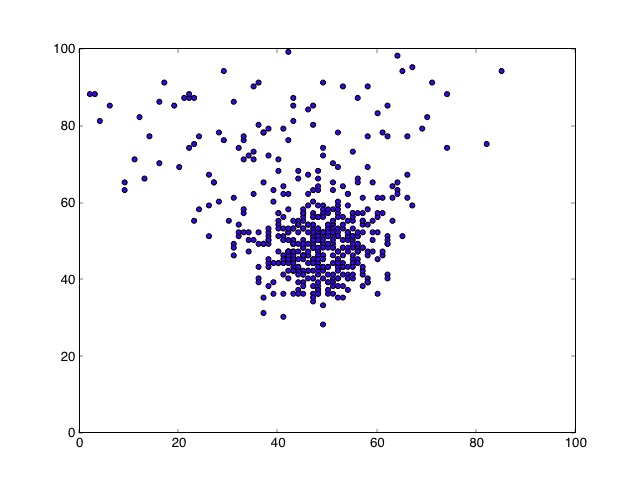
\includegraphics[width=4.5in]{scatter.jpg}
\caption{A scatter plot of runs in random 100 character subsequences, untransformed (x axis) and BW Transformed (y axis).}
\label{scatter}
\end{figure}

\subsection*{3}  The scatter plot has a roughly normal distribution across the x axis (the untransformed sequence runs), centered around 50.  This is to be expected, as runs of characters should roughly be a function of the length of the string.  But the Y axis, the Burrows -Wheeler transformed string runs, has a distribution skewed upwards.  So we know that this pattern is is very likely to generate large amounts of repeated characters, even in strings that don't have many to begin with.  This is most noticeable in the upper left hand portion of the graph.  For these data points, the original string had close to no runs, while the BWT string had almost all runs.  Additionally, the algorithm almost never decreased the number of runs in a string, as evidenced by the fact that almost all of the results lie above the identity line ($y = x$).

It is clear from these results that the BWT algorithm almost always increases runs.  In other words, in the graph,   Why might this be?

The Burrows-Wheeler Transform involves an alphabetization step in it.  If the BWT string were taken from the first column of this alphabetized array, practically every string would be full of runs.  Even though the algorithm takes the last column of these rotated strings, the last-first principle indicates that the number of runs will be much greater than otherwise would be the case.  This is, of course, one of the strengths of the algorithm with regards to lossless compression. 

\section*{Question 6: Programming exercise}
See separate submission.
\end{document} 